This section focuses on the effects of multiple users connected to the same
access point. Combined with different distances between users and the access
point, or larger numbers of users at the same distance from the access point,
the throughput, delay, and PLR are calculated.

\subsubsection{Part 1:}

This section introduces a second user to the initial system, at a distance of
100 meters from the access point, i.e. twice the distance of the initial user.
This second user was added by creating an input value which could be used to
iterate through a loop, creating new sink nodes. For each of these sink nodes, a
new source, with the corresponding listening port number was required to be
created. This can be seen within the wifi-example-sim.cc code within the
Appendices.

The throughput for both user 1 and user 2 can be seen below. The throughput of
user 2 is lower than that of user 1, due to one lost packet. This packet is
presumably lost due to the added distance from this user to the access point.

\begin{lstlisting}[language=C++, caption=Loop Snippet for adding a source and sink to
the provided code.]
  cmd.AddValue ("users", "Number of Users", users);

  Ptr<Sender> sender[users];
  Ptr<Node> appSource = NodeList::GetNode (0);
  for(int i=0; i<users; i++){
    sender[i] = CreateObject<Sender>();
    sender[i]->SetAttribute("Port", UintegerValue(1000+i));//Lisening Port of the first WiFi user
    //Code removed for the purposes of snippet
    sender[i]->SetStartTime (Seconds (0));
  }

  Ptr<Receiver> receiver[users];
  for(int i=0; i<users; i++){
    Ptr<Node> appSink = NodeList::GetNode (i+1);
    receiver[i] = CreateObject<Receiver>();
    receiver[i]->SetAttribute("Port", UintegerValue(1000+i));//Lisening Port
    appSink->AddApplication (receiver[i]);
    receiver[i]->SetStartTime (Seconds (0));

    //Set IP address of the first User to AP (source)
    string ipString = "192.168.0."+std::to_string(i+2);
    const char* ip = ipString.c_str();
    //cout << ip;
    Config::Set ("/NodeList/*/ApplicationList/"+std::to_string(i)+"/$Sender/Destination",
               Ipv4AddressValue (ip));
  }
\end{lstlisting}
\begin{gather*}
	Throughput=\frac{rxPackets*1000*8}{txTime} \\
	TP_{user_1}=\frac{5000*1000*8}{20} \\
	= 2000 Kbps \\
	TP_{user_2}=\frac{4999*1000*8}{20} \\
	= 1999.6 Kbps \\
\end{gather*}
\captionof{equation}{Average Throughput (Kbps)}

\begin{figure}[H]
	\centering
	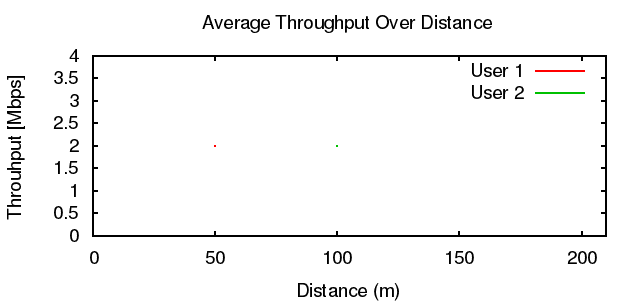
\includegraphics[width=0.8\textwidth]{images/EE500/QC/P1/Images/wifi-throughput}
	\caption{Throughput for 2 users, one at a distance of 50m, one at a
	distance of 100m}
	\label{fig:QCP1throughput}
\end{figure}

The calculations below show the difference in delay as shown in the database
(``.db'') file. There is greater delay between user 2 and the access point,
again, presumably due to the increased distance. This difference in delay
however is not shown in the output plot, possibly due to an issue in
wifi-p1qcp1.sh, which extracts the required information from the .db file using
the ``awk'' command line tool.

\begin{gather*}
	\overline{delay}=\frac{delaySum}{rxPackets} \\
	\overline{delay}_{user 1}=\frac{2224452124}{5000} \\
	= 444890.4248ns \\
	\overline{delay}_{user 2}=\frac{10823682785}{4999} \\
	= 2165169.591ns \\
\end{gather*}
\captionof{equation}{Average Delay (s)}

\begin{figure}[H]
	\centering
	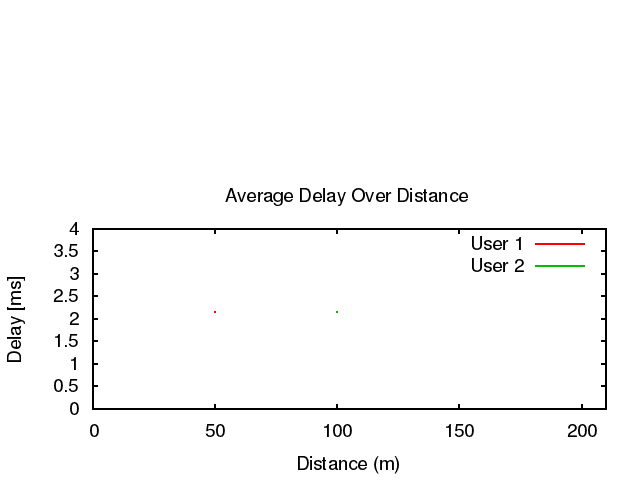
\includegraphics[width=0.8\textwidth]{images/EE500/QC/P1/Images/wifi-delay}
	\caption{Delay for 2 users, one at a distance of 50m, one at a distance
	of 100m}
	\label{fig:QCP1delay}
\end{figure}

While there is a minor difference in packet loss ratio between user 1 and user
2, this difference is so small it cannot be shown on the output graph. However,
the difference shown in the equations below is based off the database file,
which shows that there is one packet lost in the transmission between the access
point and the second user.

\begin{gather*}
	PLR=\frac{lostPackets}{rxPackets+lostPackets} \\
	PLR_{user 1}=\frac{0}{5000+0} \\
	= 0 \\
	PLR_{user 2}={1}{4999+1} \\
	= 0.0002
\end{gather*}
\captionof{equation}{Average Packet Loss Ratio}

\begin{figure}[H]
	\centering
	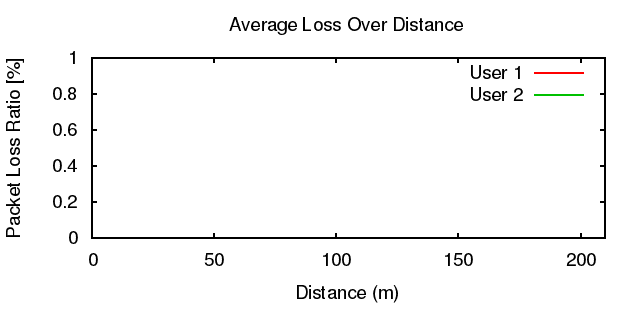
\includegraphics[width=0.8\textwidth]{images/EE500/QC/P1/Images/wifi-loss}
	\caption{Loss for 2 users, one at a distance of 50m, one at a distance
	of 100m}
	\label{fig:QCP1loss}
\end{figure}
